\chapter{Closed Cells in Sections B}
\label{ch:assignment3}

\begingroup\itshape Assignment 3 --- 19 points\endgroup

\bigskip
The three configurations (Figures~7--9 of the brief) consist of a rectangular box $5b\times2b$ with stiffeners on the top and bottom plates; $M_t$ acts CCW through CT and the stiffeners are evenly distributed (centres at $y=5b/6$, $15b/6$, $25b/6$ for three stiffeners and at $y=b/2+(i-1)b$ for five). Geometry read from the figures:
\begin{itemize}
  \item T-stiffeners (configuration 1, and the five top stiffeners of configuration 2): web height $b/2$, web thickness $t_p$, flange width $b/4$, flange thickness $2t_p$;
  \item trapezoidal stiffeners (configurations 2 and 3): crown width $b/3$ with thickness $t_p$, legs at $45^\circ$ with thickness $t_p/2$ and length $(b/4)\sqrt2$, base width $5b/6$ on the plate, height $b/4$, enclosed cell area $A_t=\tfrac12(5b/6+b/3)(b/4)=\tfrac{7}{48}b^2=0.1458\,b^2$; the small T on the crown (configuration 2) has web $b/4\times t_p$ and flange $b/4\times t_p$;
  \item configuration 3: trapezoids on top and bottom plates connected by a vertical web (thickness $t_p$, assumed) between the crowns;
  \item box plating: thickness $2t_p$ (see below).
\end{itemize}
The plating thickness of the box is not dimensioned in the figures. It was determined by reproducing the given results of configuration 3 with the multi-cell method of Assignment~2: with $2t_p$ plating the model gives $I_{p,3}=62.2\,b^3t_p$, $\tau_{max,3}=0.0271\,M_t/(b^2t_p)$ and $M_{t,3}=36.9\,b^2t_p\tau_{max}$, within 1--2\% of the given $61.558$, $0.02769$ and $36.114$ (with $t_p$ plating one would obtain $33.1\,b^3t_p$, a factor two off). The remaining difference is attributed to details of the web/crown junctions. All results below therefore use box plating $2t_p$, and the given values are used for configuration 3.

For the closed cells the Bredt--Batho relations \eqref{eq:bredt} apply; the open stiffeners contribute $I_{p,open}=\frac13\sum L_it_i^3$ and, at the common twist rate, carry the torque $G\theta'I_{p,open}$ with a linear through-thickness stress $\tau_{open}=G\theta't$.

\section{Shear flow sketch for Configurations 1 and 2}

Sketch the shear flow using arrows for Configurations 1 and 2. \textbf{(2 pts)}

\bigskip
Figure~\ref{fig:cfgflow} shows the shear flows. In configuration 1 the box is a single cell with a constant CCW shear flow; the T-stiffeners are open and carry no shear flow (only the St.\,Venant through-thickness stress). In configuration 2 the three trapezoids form three additional small cells on the bottom plate: the main cell flow $q_m$ runs CCW along the box plating and, between the trapezoid bases, along the bottom plate; each trapezoid cell has its own CCW flow $q_t$, so the base plate of the trapezoid carries $q_t$ and the legs and crown (shared between main and trapezoid cell) carry the difference $q_m-q_t$ in the sense of the main cell.

\begin{figure}[htb]
  \centering
  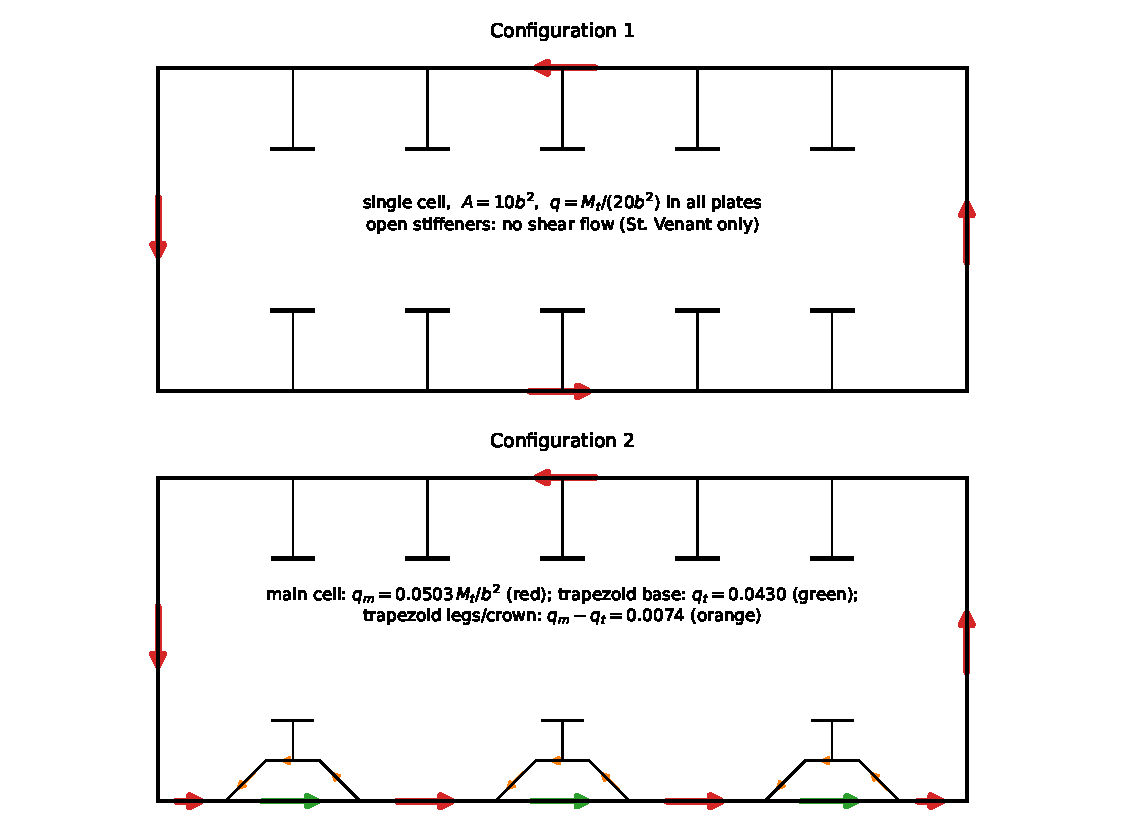
\includegraphics[width=0.95\textwidth]{figures/a3_flow}
  \caption{Shear flow (direction and relative magnitude) for configurations 1 and 2 under a CCW torsional moment; values from Question~3.3.}
  \label{fig:cfgflow}
\end{figure}

\section{T-stiffener versus L-stiffener}

Explain the consequences for the torsion stiffness contribution of open sections if a T-stiffener is exchanged for an L-stiffener, in case the web and flange dimensions remain the same. \textbf{(1 pt)}

\bigskip
The free (St.\,Venant) torsion constant of an open thin-walled profile is $I_p=\frac13\sum L_it_i^3$, i.e.\ it depends only on the lengths and thicknesses of the flat parts and not on how they are arranged. Moving the flange from the symmetric T position to the one-sided L position therefore leaves the contribution $\frac13\left(\tfrac{b}{2}t_p^3+\tfrac{b}{4}(2t_p)^3\right)=\tfrac56bt_p^3$ per stiffener unchanged. Only second-order effects differ: the junction correction (one free flange end instead of two, slightly different fillet term) and the position of the shear centre of the stiffener (at the web/flange junction in both cases, so the torque is applied identically). Consequences appear in \emph{warping} rather than in free torsion: the L-profile is asymmetric, has a (small) warping constant about its own shear centre and a larger tendency to lateral--torsional buckling (tripping) under compression, and its flange is loaded eccentrically. For the global torsion stiffness of the stiffened box these effects are negligible, and since the open contributions are anyway of order $(t_p/b)^2$ relative to the closed cell (Question~3.5), the exchange has no practical consequence for $I_p$.

\section{Shear flow components}

Calculate the shear flow components $q_i(b,t_p,M_t)$ for Configurations 1 and 2. \textbf{(4 pts)}

\bigskip
\emph{Configuration 1.} One cell with $A_1=5b\cdot2b=10b^2$ and $\oint\mathrm{d}s/t=14b/(2t_p)=7b/t_p$. Neglecting the torque carried by the open stiffeners (justified in Question~3.5; the exact fraction is $I_{p,open}/I_p\approx0.15(t_p/b)^2$):
\begin{equation}
  \boxed{\;q_1=\frac{M_t}{2A_1}=\frac{M_t}{20b^2}=0.0500\,\frac{M_t}{b^2}\;}\qquad
  I_{p,1,closed}=\frac{4A_1^2}{\oint\mathrm{d}s/t}=\frac{400b^4}{7b/t_p}=57.14\,b^3t_p .
\end{equation}

\emph{Configuration 2.} Two unknown flows: $q_m$ (main cell, $A_m=10b^2-3A_t=9.5625\,b^2$) and $q_t$ (each of the three identical trapezoid cells, $A_t=0.1458\,b^2$). Wall lengths over thickness (units $b/t_p$): box plating without the three trapezoid bases $(14-2.5)/2=5.75$; each trapezoid: legs $2\cdot0.3536/0.5=1.414$, crown $0.333/1=0.333$, base $0.833/2=0.417$. Cell equations \eqref{eq:bredt}:
\begin{align}
  \text{main:}\quad & \left[5.75+3(1.414+0.333)\right]q_m-3(1.414+0.333)\,q_t = 2\cdot9.5625\,b^2G\theta' \nonumber\\
  \text{trapezoid:}\quad & -(1.414+0.333)\,q_m+(1.414+0.333+0.417)\,q_t = 2\cdot0.1458\,b^2G\theta'
\end{align}
i.e.\ $10.99\,q_m-5.243\,q_t=19.125$, $-1.747\,q_m+2.164\,q_t=0.2917$ (per $bt_pG\theta'$), with solution $q_m=2.934$, $q_t=2.504$ ($\times bt_pG\theta'$). Then $I_{p,2,closed}=2A_mq_m+3\cdot2A_tq_t=(19.125\cdot2.934+0.875\cdot2.504)\,b^3t_p=58.30\,b^3t_p$, and per unit torque
\begin{equation}
  \boxed{\;q_m=0.0503\,\frac{M_t}{b^2},\qquad q_t=0.0430\,\frac{M_t}{b^2},\qquad q_m-q_t=0.0074\,\frac{M_t}{b^2}\ \text{(legs and crown)}\;}
\end{equation}
The trapezoid cells are so small that their flow is almost equal to that of the main cell, and the legs/crown carry only 15\% of $q_m$; the flow through the box plating ($0.0503$) is practically the single-cell value of configuration 1 ($0.0500$). Dimension check: $[q]=[M_t/b^2]=$N/m.

\section{Maximum shear stress}

\begin{enumerate}[label=\alph*.]
  \item Locate the position of maximum shear stress and obtain $\tau_{max,i}(b,t_p,M_t)$ for Configurations 1 and 2 (assuming $b\gg t_p$). \textbf{(3 pts)}

  With $b\gg t_p$ the stress in the open stiffeners, $\tau_{open}=G\theta't_{max}=2t_p\,M_t/I_p=0.035\,(t_p/b)\,M_t/(b^2t_p)$, is a factor $1.4\,t_p/b\ll1$ smaller than in the closed walls, and the closed walls carry the full torque. Configuration~1: uniform stress in all four box plates,
  \begin{equation}
    \boxed{\;\tau_{max,1}=\frac{q_1}{2t_p}=\frac{M_t}{40\,b^2t_p}=0.0250\,\frac{M_t}{b^2t_p}\;}\qquad(\text{everywhere in the box plating}).
  \end{equation}
  Configuration~2: box plating $\tau=0.0503/2=0.0252$; trapezoid base $0.0430/2=0.0215$; legs ($t_p/2$) $0.0074/0.5=0.0148$; crown $0.0074$. Hence
  \begin{equation}
    \boxed{\;\tau_{max,2}=0.0252\,\frac{M_t}{b^2t_p}\;}\qquad\text{in the box plating (sides, top and bottom plate between the trapezoids)}.
  \end{equation}

  \item Compare the outcomes of configuration 1 and 2 to the (given) outcome of configuration 3 and discuss the differences. \textbf{(2 pts)}

  Configuration 3: $\tau_{max,3}=0.02769\,M_t/(b^2t_p)$, i.e.\ 11\% higher than configurations 1 ($0.0250$) and 2 ($0.0252$), which are practically equal. In configurations 1 and 2 the torque is carried by one large cell with a nearly uniform shear flow $M_t/(2A)$ in $2t_p$ plating. In configuration 3 the webs divide the box into four cells in series across the breadth and the six trapezoids into small cells; the cell flows differ (larger in the two central cells than in the outer cells), so that the plating between the central trapezoids carries a higher net flow ($0.054\,M_t/b^2$ in the own model) than the average $0.05\,M_t/b^2$. The subdivision thus concentrates shear flow in the middle of the top and bottom plates and raises the peak stress, while the total enclosed area (and therefore the average flow) is unchanged. In the own model of configuration 3 the thin legs ($t_p/2$) of the outer trapezoids come close to the plating stress ($0.025$), which shows that thin walls of small cells adjacent to large cells are potential hot spots.
\end{enumerate}

\section{Specific torsion stiffness and strength}

\begin{enumerate}[label=\alph*.]
  \item Calculate the (specific) torsion stiffness $I_{p,i}(b,t_p)$ and strength $M_{t,i}(b,t_p,\tau_{max})$ for Configurations 1 and 2. \textbf{(3 pts)}

  Closed parts from Question~3.3; open parts $\frac13\sum Lt^3$: configuration 1 has ten T's of $\frac13(\tfrac b2t_p^3+\tfrac b4\cdot8t_p^3)=\tfrac56bt_p^3$, configuration 2 five large T's and three small T's of $\frac13(\tfrac b4+\tfrac b4)t_p^3=\tfrac16bt_p^3$:
  \begin{align}
    I_{p,1}&=57.14\,b^3t_p+8.33\,bt_p^3=57.14\,b^3t_p\left[1+0.146\,(t_p/b)^2\right]\approx\boxed{57.1\,b^3t_p}\\
    I_{p,2}&=58.30\,b^3t_p+4.67\,bt_p^3=58.30\,b^3t_p\left[1+0.080\,(t_p/b)^2\right]\approx\boxed{58.3\,b^3t_p}
  \end{align}
  Strength (torque at which $\tau_{max}$ is reached in the governing wall, Question~3.4a):
  \begin{equation}
    M_{t,1}=\frac{b^2t_p\tau_{max}}{0.0250}=\boxed{40.0\,b^2t_p\tau_{max}},\qquad
    M_{t,2}=\frac{b^2t_p\tau_{max}}{0.02516}=\boxed{39.7\,b^2t_p\tau_{max}} .
  \end{equation}
  Order-of-magnitude check: $M_{t,1}=2A\,t\,\tau_{max}=2\cdot10b^2\cdot2t_p\tau_{max}=40\,b^2t_p\tau_{max}$ (Bredt's first formula), and $I_{p,1}=4A^2t/\oint\mathrm{d}s$ (Bredt's second formula).

  \item Compare the outcomes of Configurations 1 and 2 to the (given) outcome of Configuration 3 and discuss the origin of possible differences. \textbf{(2 pts)}

  \begin{center}\small
  \begin{tabular}{lccc}
    \toprule
     & config.\ 1 & config.\ 2 & config.\ 3 (given) \\
    \midrule
    $I_p$ [$b^3t_p$] & 57.1 & 58.3 & 61.6 \\
    $\tau_{max}$ [$M_t/(b^2t_p)$] & 0.0250 & 0.0252 & 0.0277 \\
    $M_t$ [$b^2t_p\tau_{max}$] & 40.0 & 39.7 & 36.1 \\
    \bottomrule
  \end{tabular}
  \end{center}
  \emph{Stiffness.} Configuration 3 is 8\% stiffer than 1 and 6\% stiffer than 2. All three configurations enclose the same total area $10b^2$ with the same $2t_p$ plating, so the single-cell value $57.1\,b^3t_p$ is the base value. Adding closed walls inside a closed section never reduces $I_p$: the webs, legs and crowns of configuration 3 provide additional parallel shear paths, the cell flows redistribute (larger flows in the central cells) and the effective $\oint\mathrm{d}s/t$ seen by the flow decreases, which yields the 8\% gain. In configuration 2 only the three small bottom trapezoids are closed, which gives 2\%; its open T-stiffeners, like all stiffeners of configuration 1, contribute only $\mathcal O\big((t_p/b)^2\big)$. \emph{Strength.} Configuration 3 is the weakest (10\% lower than 1) because the subdivision into cells with unequal flows produces a local peak in the plating between the central trapezoids (Question~3.4b), whereas the single-cell configurations load their plating uniformly. Thus, for the same plating, converting open stiffeners into closed cells increases the stiffness noticeably, but may reduce the torsional strength when the cell arrangement produces uneven shear flows; the amount of stiffener material also differs between the configurations, so the comparison is not at equal weight.

  \item For Configurations 1 and 2 split the relative stiffness and strength contributions for the open and closed parts and discuss the differences. \textbf{(2 pts)}

  At the common twist rate $\theta'$ the torque splits in proportion to the torsion constants, $M_{closed}:M_{open}=I_{p,closed}:I_{p,open}$:
  \begin{center}\small
  \begin{tabular}{lcc}
    \toprule
     & config.\ 1 & config.\ 2 \\
    \midrule
    $I_{p,closed}$ & $57.14\,b^3t_p$ & $58.30\,b^3t_p$ \\
    $I_{p,open}$ & $8.33\,bt_p^3$ & $4.67\,bt_p^3$ \\
    $I_{p,open}/I_{p,closed}$ & $0.146\,(t_p/b)^2$ & $0.080\,(t_p/b)^2$ \\
    e.g.\ $b/t_p=50$ & $5.8\times10^{-5}$ & $3.2\times10^{-5}$ \\
    $\tau_{open,max}/\tau_{closed,max}$ & $1.40\,t_p/b$ & $1.36\,t_p/b$ \\
    \bottomrule
  \end{tabular}
  \end{center}
  The open stiffeners carry a fraction $\mathcal O\big((t_p/b)^2\big)$ of the torque, i.e.\ well below $10^{-3}$ for any realistic plate slenderness, and their contribution to the stiffness is negligible. For strength the open parts are irrelevant as well: their maximum stress is $G\theta't_{max}$, a factor $\approx1.4\,t_p/b$ (a few per cent) below the stress in the closed walls, so the closed cells govern both stiffness and strength. In configuration 2 the ``open'' share is smaller than in configuration 1 because three of the bottom stiffeners have become closed trapezoids and the small T's have thinner flanges; the closed share is correspondingly 2\% larger. The practical conclusion is that open stiffeners are provided for local plate bending and buckling, not for torsion, and that torsional stiffness must come from closed cells (hatch covers, wing tanks, double bottom, torsion boxes).
\end{enumerate}
